\documentclass[12pt,a4paper]{article}

% Language setting
\usepackage[spanish]{babel}
\providecommand{\keywords}[1]
{
  \small	
  \textbf{Keywords:} #1
}

%Paquete para insertar código python
\usepackage{listings}
\lstdefinestyle{mystyle}{
    language=Python,
    basicstyle=\small\ttfamily,
    keywordstyle=\color{blue},
    commentstyle=\color{green},
    stringstyle=\color{purple},
    breaklines=true,
    showstringspaces=false,
    numbers=left,
    numberstyle=\tiny,
    frame=lines
}

\lstset{style=mystyle}
% Set page size and margins
% Replace `letterpaper' with `a4paper' for UK/EU standard size
\usepackage[letterpaper,top=2cm,bottom=2cm,left=3cm,right=3cm,marginparwidth=1.75cm]{geometry}

% Useful packages
\usepackage{cite}
\usepackage{amsmath}
\usepackage{graphicx}
\usepackage[colorlinks=true, allcolors=blue]{hyperref}

\title{Algoritmo de Kruskal e implementación en Python}
\author{Cristian Lopera \and Andrea Argumedo  }

\begin{document}
\maketitle

\begin{abstract}
Este artículo explora el algoritmo de Kruskal, el cual es una herramienta fundamental en la teoría de grafos para encontrar árboles de expansión mínima. Se realiza una definición del algoritmo de Kruskal, A través de un ejemplo sencillo y aplicable, se muestra cómo el algoritmo selecciona aristas para construir una red eficiente y que no tenga ciclos, se continua con una explicaión detallada de como realizar la implementación del algoritmo de Kruskal usando el lenguaje de prograamación Python.Este artículo se presenta como una valiosa guía para aquellos que buscan no solo comprender el algoritmo de Kruskal desde un punto de vista teórico, sino también aplicarlo en proyectos de programación del mundo real.

\end{abstract}

\keywords {Algoritmo, \and Python, \and Lenguaje de Programación, \and grafos, \and optimización.}

\section{Introduction}

El algoritmo de Kruskal, desarrollado por Joseph Kruskal, es un método eficiente para encontrar el árbol de expansión mínima en un grafo ponderado no dirigido. La problemática a la que responde este algoritmo es fundamental en teoría de grafos y aplicaciones prácticas como redes de comunicación, planificación de rutas y diseño de circuitos. El algoritmo se centra en seleccionar aristas ordenadas por peso de menor a mayor, asegurando de que no se formen ciclos. Este enfoque garantiza la construcción de un árbol que conecta todos los vértices del grafo con la longitud total mínima.

\section{Algoritmo de Kruskal}

\subsection{Definición}

El algoritmo de Kruskal es un algoritmo de la teoría de grafos para encontrar un árbol recubridor mínimo en un grafo conexo y ponderado. Es decir, busca un subconjunto de aristas que, formando un árbol, incluyen todos los vértices y donde el valor de la suma de todas las aristas del árbol es el mínimo. Si el grafo no es conexo, entonces busca un árbol de expansión mínimo. Este algoritmo toma su nombre de Joseph Kruskal, quien lo publicó por primera vez en 1956\cite{Kruskal}.

Un árbol de expansión mínimo es un tipo especial de árbol que minimiza las longitudes (o «pesos») de los bordes del árbol. Un ejemplo es una compañía de cable que quiere tender línea a múltiples vecindarios; al minimizar la cantidad de cable tendido, la compañía de cable ahorrará dinero \cite{arbol}.

Para entender de una manera más simple lo que se puede lograr con la implementación de este algoritmo, se muestra un ejemplo real.
Imaginemos que tenemos un mapa con ciudades (vértices) y caminos entre ellas (aristas), y cada camino tiene una longitud (peso). Queremos encontrar la forma más barata de conectar todas las ciudades. Eso se llama un "árbol de expansión mínima"; observando la figura \ref{fig:ejemplo1} vamos a suponer que los números encerrados en círculos azules son las ciudades.

\begin{figure}[h!]
\centering
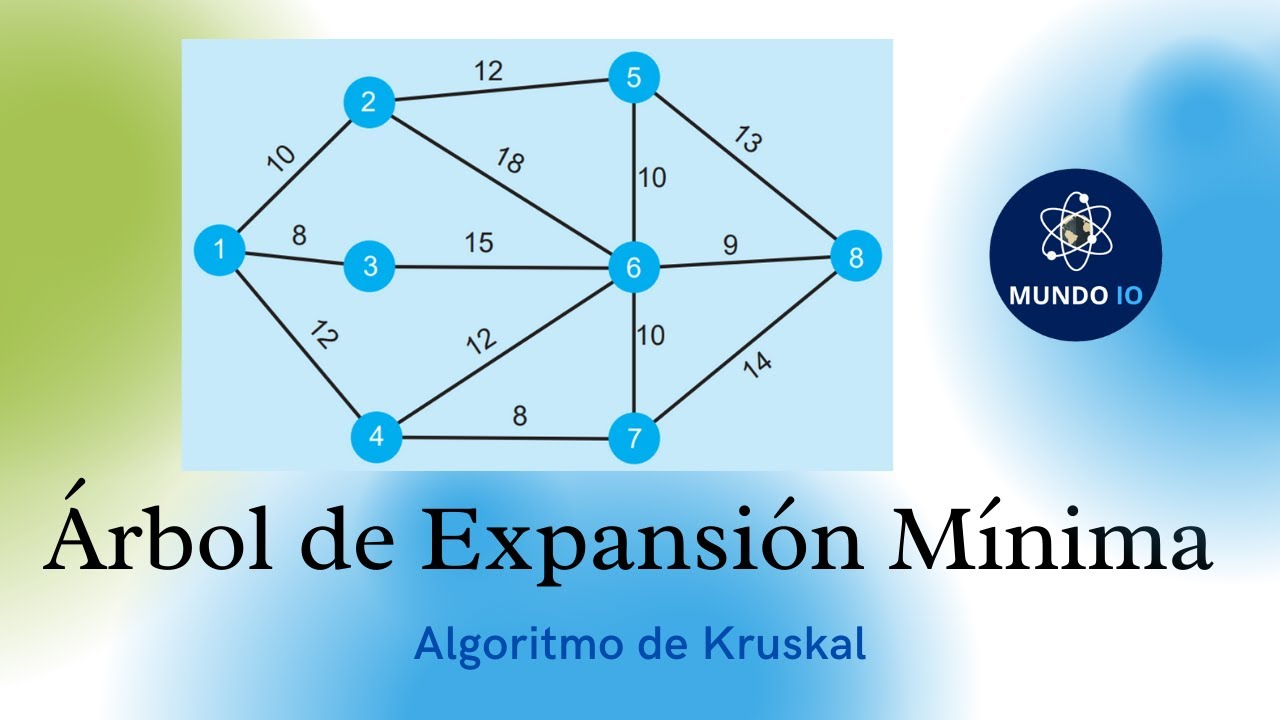
\includegraphics[width=0.8\textwidth]{Ejemplo1.jpg}
\caption{\label{fig:ejemplo1}Muestra diferentes puntos de una red interconectados \cite{ImagenEjemplo}.}
\end{figure}

En la ecuación \ref{ecuación1} se muestra la sumatoria de todos los "Pesos" de las conexiones antes de implementar el algoritmo de Kruskal:

\begin{equation}
\label{ecuación1}
    Total = 10+12+13+14+8+12+8+15+9+18+10+10+12 = 151
\end{equation}

El algoritmo de Kruskal hace lo siguiente:

\begin{enumerate}
    \item Preparación: Tienes todas las posibles carreteras (aristas) entre las ciudades y sus longitudes (pesos). Ordenas estas carreteras de la más corta a la más larga.
    \item Comienzo: Inicias sin ninguna carretera construida y cada ciudad es una "isla" independiente.
    \item Construcción: Comienzas a agregar las carreteras más cortas. Si una carretera no forma un ciclo (no conecta dos ciudades que ya están conectadas), la agregas a tu red y fusionas esas dos ciudades. Repites esto hasta que todas las ciudades están conectadas.
    \item Resultado: Al final, obtienes una red de carreteras (un árbol de expansión mínima) que conecta todas las ciudades de la manera más corta posible.
\end{enumerate}

En la figura \ref{fig:ejemplo2} se muestra la forma más económica para conectar todas las ciudades, la cual estaría señalada por las líneas rojas, donde se observan que todos los puntos quedan interconectados:


\begin{figure}[h!]
\centering
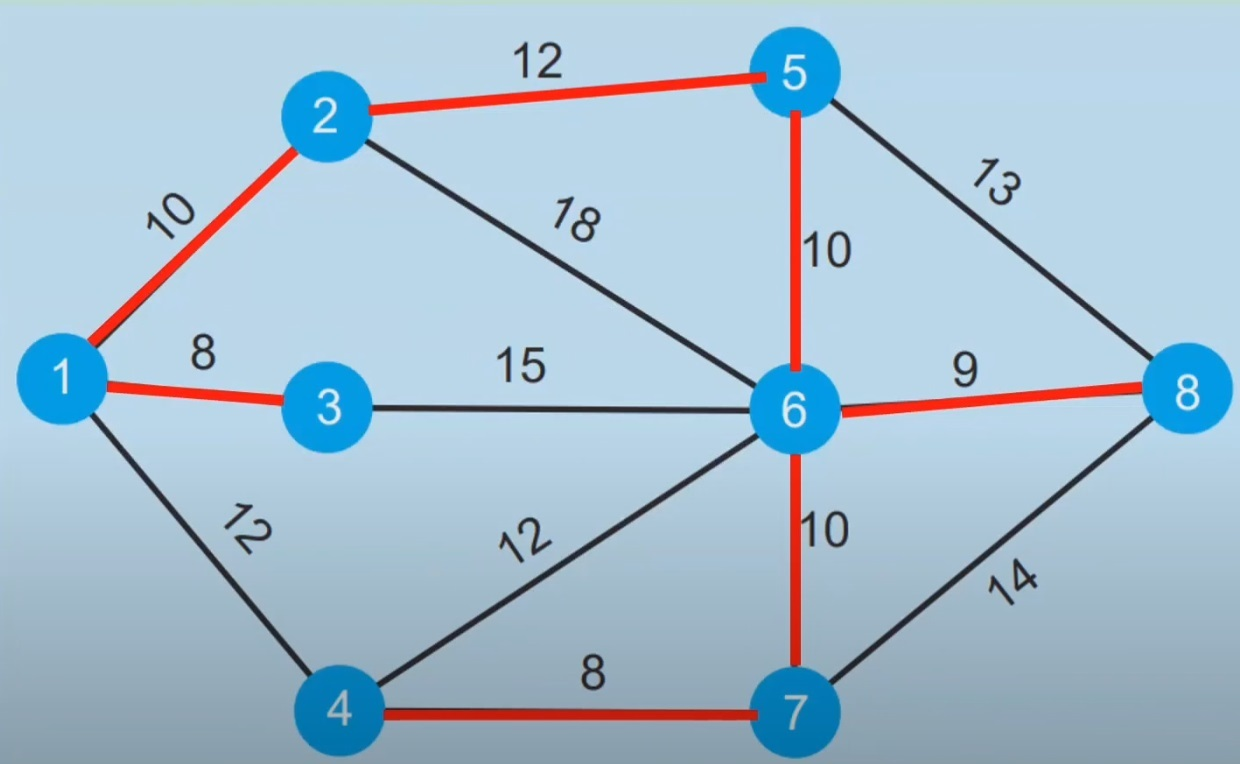
\includegraphics[width=0.8\textwidth]{Ejemplo2.jpg}
\caption{\label{fig:ejemplo2}Implementación del algoritmo de Kruskal}
\end{figure}
\newpage
En la ecuación \ref{ecuación2} se muestra la sumatoria de todos los "Pesos" de las conexiones después de implementar el algoritmo de Kruskal

\begin{equation}
\label{ecuación2}
    Total = 8+10+12+10+9+10+8 = 67
\end{equation}

\subsection{Implementación en Python}

A continuación, se presenta la implementación del algoritmo de Kruskal utilizando el lenguaje de progración \textbf{Python}.

Primeramente se tiene una clase  \textbf{class Graph} la cual contendrá todo el código, la cual está conformoda por un constructor y funciones \textbf{def add\_edge, def search , def apply\_union y def kruskal} las cuales permiten añadir, correlacionar y unir conjuntos para obtener de manera óptima la forma más económica de unir todos los puntos \cite{algoritmo}.

\begin{lstlisting}[caption={Algoritmo de Kruskal en Python}, label={lst:python}]
    class Graph:
    def __init__(self, vertex):
        self.V = vertex
        self.graph = []
 
    def add_edge(self, u, v, w):
        self.graph.append([u, v, w])
 
 
    def search(self, parent, i):
        if parent[i] == i:
            return i
        return self.search(parent, parent[i])
 
    def apply_union(self, parent, rank, x, y):
        xroot = self.search(parent, x)
        yroot = self.search(parent, y)
        if rank[xroot] < rank[yroot]:
            parent[xroot] = yroot
        elif rank[xroot] > rank[yroot]:
            parent[yroot] = xroot
        else:
            parent[yroot] = xroot
            rank[xroot] += 1
 
  
    def kruskal(self):
        result = []
        i, e = 0, 0
        self.graph = sorted(self.graph, key=lambda item: item[2])
        parent = []
        rank = []
        for node in range(self.V):
            parent.append(node)
            rank.append(0)
        while e < self.V - 1:
            u, v, w = self.graph[i]
            i = i + 1
            x = self.search(parent, u)
            y = self.search(parent, v)
            if x != y:
                e = e + 1
                result.append([u, v, w])
                self.apply_union(parent, rank, x, y)
        for u, v, weight in result:
            print("Tramo desde ",u, " hasta ", v,end =" ")
            print(":",weight)
 
g = Graph(5)
g.add_edge(0, 1, 8)
g.add_edge(0, 2, 5)
g.add_edge(1, 2, 9)
g.add_edge(1, 3, 11)
g.add_edge(2, 3, 15)
g.add_edge(2, 4, 10)
g.add_edge(3, 4, 7)
g.kruskal()

\end{lstlisting}

Primero se define la clase \textbf{Graph}, la cual contiene las siguientes funciones:
\newline

\textbf{\_\_init\_\_}: Inicializa la clase con el número de vértices (V) y una lista graph que almacenará las aristas del grafo.
\newline

\textbf{add\_edge}: Agrega una arista al grafo con los vértices u y v y su peso w.
\newline

\textbf{search}: Función de búsqueda utilizada para encontrar el conjunto al que pertenece un vértice dado.
\newline

\textbf{apply\_union}: Realiza la unión de dos conjuntos, teniendo en cuenta la clasificación (rank) para optimizar la unión.
\newline

Método \textbf{kruskal}:

\begin{itemize}
    \item \textbf{Inicialización}: Inicializa variables (result, i, y e) y ordena las aristas del grafo por peso.
    \item \textbf{Unión de conjuntos}: Itera sobre las aristas ordenadas, realizando la unión de conjuntos si los extremos (u y v) no están en el mismo conjunto.
    \item \textbf{Resultado}: Imprime las aristas del árbol de expansión mínima junto con sus pesos.
\end{itemize}

Por último se Se instancia la clase \textbf{Graph} con 5 vértices tabla \ref{tab: tabla1}, se agregan aristas al grafo, se llama al método kruskal para encontrar el árbol de expansión mínima .
\newline

\begin{table}[H]
\centering
\begin{tabular}{|c|c|c|}
\hline
\textbf{Vértice}  & \textbf{Peso}   \\ \hline
0 - 1 & 8  \\
0 - 2 & 5  \\
1 - 2 & 9  \\
1 - 3 & 11 \\
2 - 3 & 15 \\
2 - 4 & 10 \\
3 - 4 & 7 \\ \hline
\end{tabular}
\caption{Vertices con sus respectivos pesos.}
\label{tab: tabla1}
\end{table}

Por último se muestra el árbol de expansión mínima en la tabla \ref{tab: tabla2}.

\begin{table}[H]
\centering
\begin{tabular}{|c|c|c|}
\hline
\textbf{Vértice}  & \textbf{Peso}   \\ \hline

0 - 2 & 5  \\
3 - 4 & 7 \\
0 - 1 & 8  \\
2 - 4 & 10 \\ \hline
\end{tabular}
\caption{Resultado ejecución código python.}
\label{tab: tabla2}
\end{table}

De esta manera, usando Python se puede obtener de forma sencilla la implementación del algoritmo de Kruskal, facilitando la creación de estructuras eficientes de árboles de expansión mínima.

\section{Conslusión}

En conclusión, el artículo ha explorado el algoritmo de Kruskal, destacando su importancia en la teoría de grafos y su aplicación práctica en la optimización de redes. Desde la introducción de los conceptos fundamentales de árboles de expansión mínima hasta un ejemplo sencillo pero revelador, se ha proporcionado una comprensión clara del algoritmo.

La guía detallada de implementación en Python ha demostrado que, gracias a la sintaxis limpia y la versatilidad del lenguaje, la traducción de la teoría a la práctica es accesible incluso para aquellos con poca experiencia en programación. La inclusión de un entorno de desarrollo en LaTeX con el paquete listings ha permitido presentar el código de una manera estéticamente agradable y fácil de entender en el contexto del artículo.

En última instancia, el algoritmo de Kruskal se presenta no solo como un concepto académico, sino como una herramienta valiosa y aplicable en la informática y la ingeniería.

\bibliographystyle{ieeetr}%%%% 
\bibliography{Referencias}

\end{document}